% Compile with XeLaTeX on Overleaf/TeX Live.
\documentclass[11pt,a4paper]{article}

\usepackage[a4paper,margin=1.8cm]{geometry}
\usepackage{fontspec}
\setmainfont{Times New Roman}
\setsansfont{Arial}
\usepackage{graphicx}
\usepackage{booktabs}
\usepackage{tabularx}
\usepackage{array}
\usepackage{enumitem}
\usepackage{xcolor}
\usepackage{hyperref}
\usepackage{caption}
\usepackage{float}
\usepackage{url}
\usepackage{xurl}
\usepackage{listings}

\graphicspath{{outputs/figures/}{../outputs/figures/}}
\hypersetup{
  colorlinks=true,
  linkcolor=black,
  urlcolor=blue,
  citecolor=black
}

\setlength{\parskip}{4pt}
\setlength{\parindent}{0pt}
\emergencystretch=3em
\setlist[itemize]{leftmargin=1.25em,itemsep=1pt,topsep=2pt}
\setlist[enumerate]{leftmargin=1.4em,itemsep=1pt,topsep=2pt}
\captionsetup{font=small,labelfont=bf}
\renewcommand{\arraystretch}{1.12}

% ====== Thong tin can sua ======
\newcommand{\TenDeTai}{Đánh giá tránh vật cản UAV dựa trên quỹ đạo, nhãn rủi ro và dữ liệu đa cảm biến trên ODA Dataset}
\newcommand{\SinhVien}{Nguyễn Thành Lâm}
\newcommand{\Mentor}{[Họ và tên mentor]}
\newcommand{\DonViMentor}{[Đơn vị mentor hướng dẫn]}
\newcommand{\EmailMentor}{[email mentor hướng dẫn]}

\begin{document}

\begin{center}
{\Large\bfseries \TenDeTai}\\[4pt]
{\normalsize \SinhVien, \Mentor\textsuperscript{1}}\\
{\small \textsuperscript{1}\DonViMentor{} -- \EmailMentor}
\end{center}

\vspace{-2mm}
\section*{Tóm tắt}
Đề tài xây dựng một pipeline nhẹ cho bài toán phát hiện nguy cơ va chạm và đánh giá tránh vật cản của Micro Air Vehicle (MAV) trong môi trường trong nhà/GNSS-denied. Thay vì bắt đầu từ ROS, Gazebo hoặc huấn luyện mô hình nặng, sinh viên tập trung khai thác dữ liệu CSV/metadata của ODA Dataset, tái dựng quỹ đạo MAV từ OptiTrack, biểu diễn vật cản, tạo nhãn rủi ro theo clearance và so sánh quỹ đạo thật với các planner baseline. Kết quả ban đầu gồm: tóm tắt cấu trúc dữ liệu, hình quỹ đạo--vật cản, bảng metric benchmark, so sánh human/straight-line/geometric bypass/A*/RRT/RRT*/MPPI, video RGB--radar--IMU--depth--safety map--trajectory, và kế hoạch mở rộng lên nhiều trial hơn.

\section{Giới thiệu chung}
UAV/MAV hoạt động trong nhà thường không có GNSS, dễ gặp các vật cản mảnh như cột, dây hoặc khung cửa. Bài toán phát hiện và tránh vật cản vì vậy cần không chỉ nhận biết môi trường mà còn phải đánh giá nguy cơ va chạm theo thời gian. ODA Dataset cung cấp các thử nghiệm MAV bay trong indoor với RGB camera, event camera, radar 24 GHz, IMU và OptiTrack ground truth, phù hợp để xây dựng pipeline đánh giá an toàn dựa trên dữ liệu thực \cite{odaGithub,oda4tu,odaPaper}.

Mục tiêu của đề tài là tạo ra một bộ kết quả đầu tiên có thể kiểm chứng được: đọc dữ liệu ODA ở mức CSV/metadata, tái dựng quỹ đạo và vị trí vật cản, tính khoảng cách an toàn, phát hiện safety-distance violation, và tạo trực quan hóa định tính đa cảm biến. Đóng góp chính của sinh viên gồm:
\begin{itemize}
  \item Thiết kế pipeline Python nhẹ, không phụ thuộc ROS/Gazebo, có thể chạy trên laptop cá nhân.
  \item Chuẩn hóa cách đọc metadata nhiều vật cản và quy ước hệ trục OptiTrack của ODA.
  \item Đề xuất bộ metric ban đầu cho collision-risk analysis: minimum distance, boundary clearance, violation, closest-approach time, path length và computation time.
  \item Xây dựng nhãn rủi ro theo thời gian gồm safe, warning, danger và collision, kèm nhãn future-risk trong cửa sổ 1 giây.
  \item So sánh quỹ đạo người lái với các baseline tránh vật cản: straight-line, geometric bypass, A* grid planner, RRT, RRT* và MPPI Python nhẹ.
  \item Tạo video định tính 3/5/6 panel kết hợp RGB, monocular predicted depth, radar FFT, IMU, safety map và trajectory để minh chứng kết quả.
\end{itemize}

\section{Nội dung và phương pháp}
\subsection{Dữ liệu và quy trình}
Pipeline sử dụng các sample public kèm GitHub của ODA Dataset, gồm sample 3, 10 và 345. File \texttt{trial\_overview.csv} được dùng để lấy số lượng vật cản, tọa độ vật cản, điều kiện ánh sáng và cờ video. Các file \texttt{optitrack.csv}, \texttt{imu.csv}, \texttt{radar.csv} và \texttt{.avi} được dùng cho từng sample khi cần video định tính. Đồng thời, sinh viên đã tạo manifest 20 trial mục tiêu cân bằng giữa một vật cản và hai vật cản để mở rộng benchmark sau khi có full dataset từ 4TU.

\begin{table}[H]
\centering
\small
\caption{Tóm tắt dữ liệu ODA được khai thác trong pipeline.}
\begin{tabularx}{0.96\linewidth}{>{\bfseries}l X}
\toprule
Hạng mục & Giá trị \\
\midrule
Số trial ID trong metadata & 1369 \\
Số dòng trong \texttt{trial\_overview.csv} & 1997, do trial hai vật cản có hai dòng tọa độ \\
Trial local đã xử lý & 3, 10, 345 \\
Manifest mở rộng & 20 trial mục tiêu; hiện 3/20 trial có đủ OptiTrack/RGB/radar/IMU tại local \\
Trial có 1 vật cản / 2 vật cản & 704 / 628 \\
Trial thiếu tọa độ vật cản & 37, tương ứng vùng sample 593--629 \\
Quy ước mặt phẳng bay & Ground plane = OptiTrack \(x\) và \(z\); chiều cao = OptiTrack \(y\) \\
\bottomrule
\end{tabularx}
\end{table}

\subsection{Metric đánh giá an toàn}
Vật cản được mô hình hóa là hình trụ bán kính \(r=0.20\,m\), theo script visualization gốc của ODA. Với mỗi thời điểm \(t_i\), khoảng cách từ MAV tới vật cản gần nhất được tính trên mặt phẳng \(x\)--\(z\):
\[
d_i = \min_j \left\|\mathbf{p}_i - \mathbf{o}_j\right\|_2,\quad
c_i = d_i - r
\]
trong đó \(\mathbf{p}_i\) là vị trí MAV, \(\mathbf{o}_j\) là vị trí vật cản, và \(c_i\) là clearance tới biên vật cản. Một trial bị xem là vi phạm khoảng cách an toàn nếu \(\min_i c_i < 0.50\,m\). Thời điểm closest approach là \(t_{i^\ast}\) với \(i^\ast=\arg\min_i c_i\).

\subsection{Trực quan hóa đa cảm biến}
Sinh viên xây dựng video định tính theo ba mức:
\begin{enumerate}
  \item \textbf{3 panel}: RGB camera, safety-distance map hình học và quỹ đạo OptiTrack.
  \item \textbf{5 panel}: thêm radar FFT từ tín hiệu radar 24 GHz và đồ thị IMU rolling window.
  \item \textbf{6 panel}: thêm monocular predicted depth từ DPT-Hybrid/MiDaS \cite{dptModel,dptPaper}. Depth panel hiện là relative depth định tính, chưa được hiệu chuẩn sang mét.
\end{enumerate}
Cách tiếp cận này giúp sản phẩm có minh chứng thị giác tương tự các demo multi-sensor nhưng vẫn giữ trọng tâm ở xử lý dữ liệu nhẹ, có thể tái lập nhanh.

\section{Kết quả thực hiện}
\subsection{Sản phẩm phần mềm}
Mã nguồn đã được tổ chức theo các module:
\begin{itemize}
  \item \texttt{src/oda\_io.py}: đọc metadata, OptiTrack, IMU và radar FFT.
  \item \texttt{src/metrics.py}: tính distance, clearance, violation, closest approach và path length.
  \item \texttt{src/risk.py}: tạo nhãn rủi ro theo clearance và nhãn future-risk theo horizon.
  \item \texttt{src/planners/}: triển khai straight-line, geometric bypass, A* grid planner, RRT, RRT* và MPPI.
  \item \texttt{src/visualize.py}: vẽ trajectory, obstacle radius, safety boundary và clearance theo thời gian.
  \item \texttt{experiments/benchmark\_oda.py}: xuất bảng metric và hình tĩnh.
  \item \texttt{experiments/batch\_benchmark\_planners.py}: benchmark nhiều trial và xuất bảng so sánh planner.
  \item \texttt{experiments/make\_qualitative\_video.py}: render video định tính nhiều panel.
  \item \texttt{experiments/cache\_monocular\_depth.py}: cache monocular relative depth từ RGB video.
\end{itemize}

\subsection{Kết quả định lượng ban đầu}
\begin{table}[H]
\centering
\small
\caption{Benchmark metric ban đầu với obstacle radius \(0.20\,m\) và safety clearance \(0.50\,m\).}
\begin{tabular}{ccccccc}
\toprule
Sample & Số vật cản & Min center (m) & Min clearance (m) & Closest time (s) & Collision & Violation \\
\midrule
3 & 1 & 0.6348 & 0.4348 & 6.4250 & Không & Có \\
10 & 1 & 1.0300 & 0.8300 & 9.3250 & Không & Không \\
345 & 2 & 1.1689 & 0.9689 & 8.6875 & Không & Không \\
\bottomrule
\end{tabular}
\end{table}

Sample 3 là trường hợp đáng chú ý vì MAV không va chạm trực tiếp nhưng đi vào vùng safety clearance \(0.50\,m\). Sample 345 có hai vật cản và MAV tránh an toàn với minimum boundary clearance \(0.9689\,m\). Thời gian tính metric cho từng trial ở mức dưới \(1\,ms\), phù hợp để mở rộng thành benchmark nhanh cho nhiều trial hơn.

\begin{figure}[H]
\centering
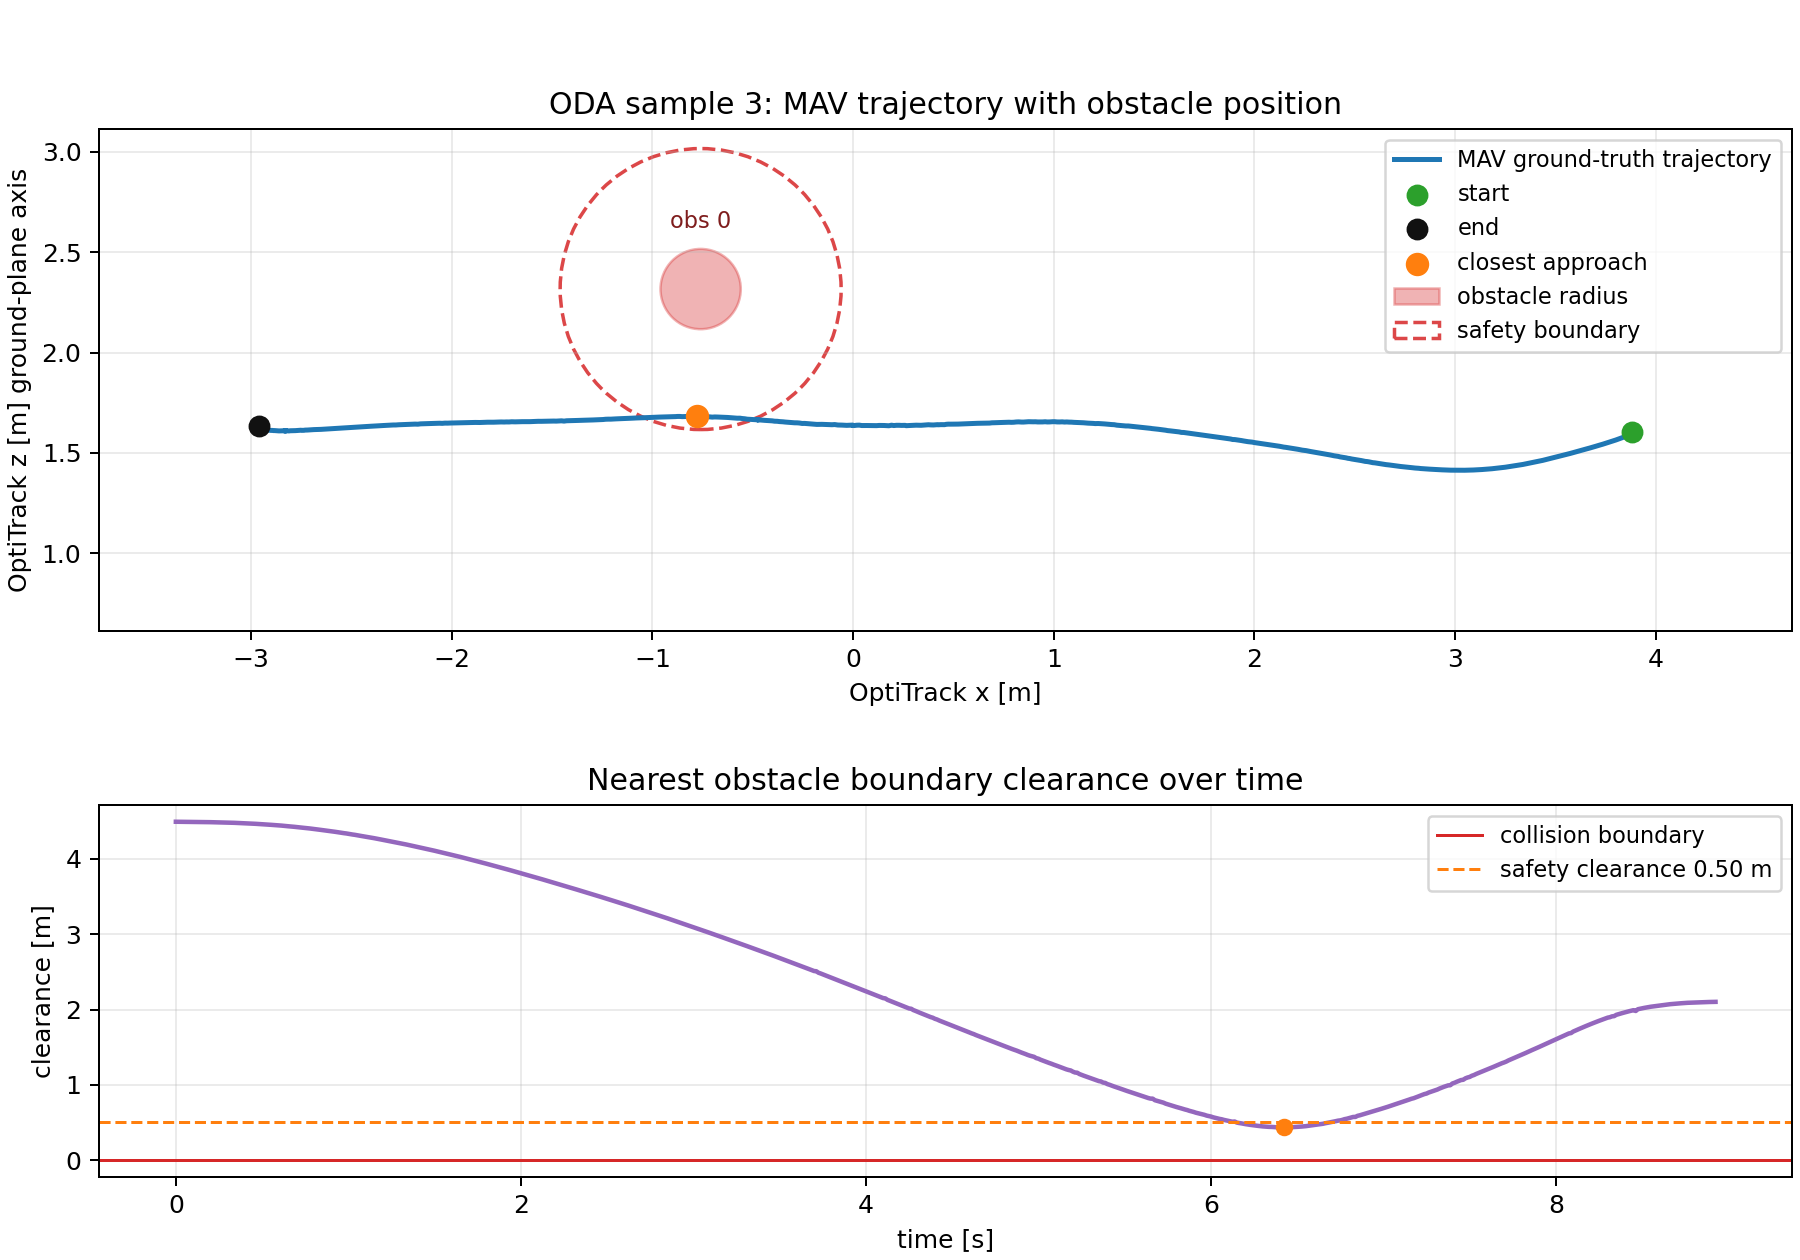
\includegraphics[width=0.49\linewidth]{trajectory_sample_3.png}
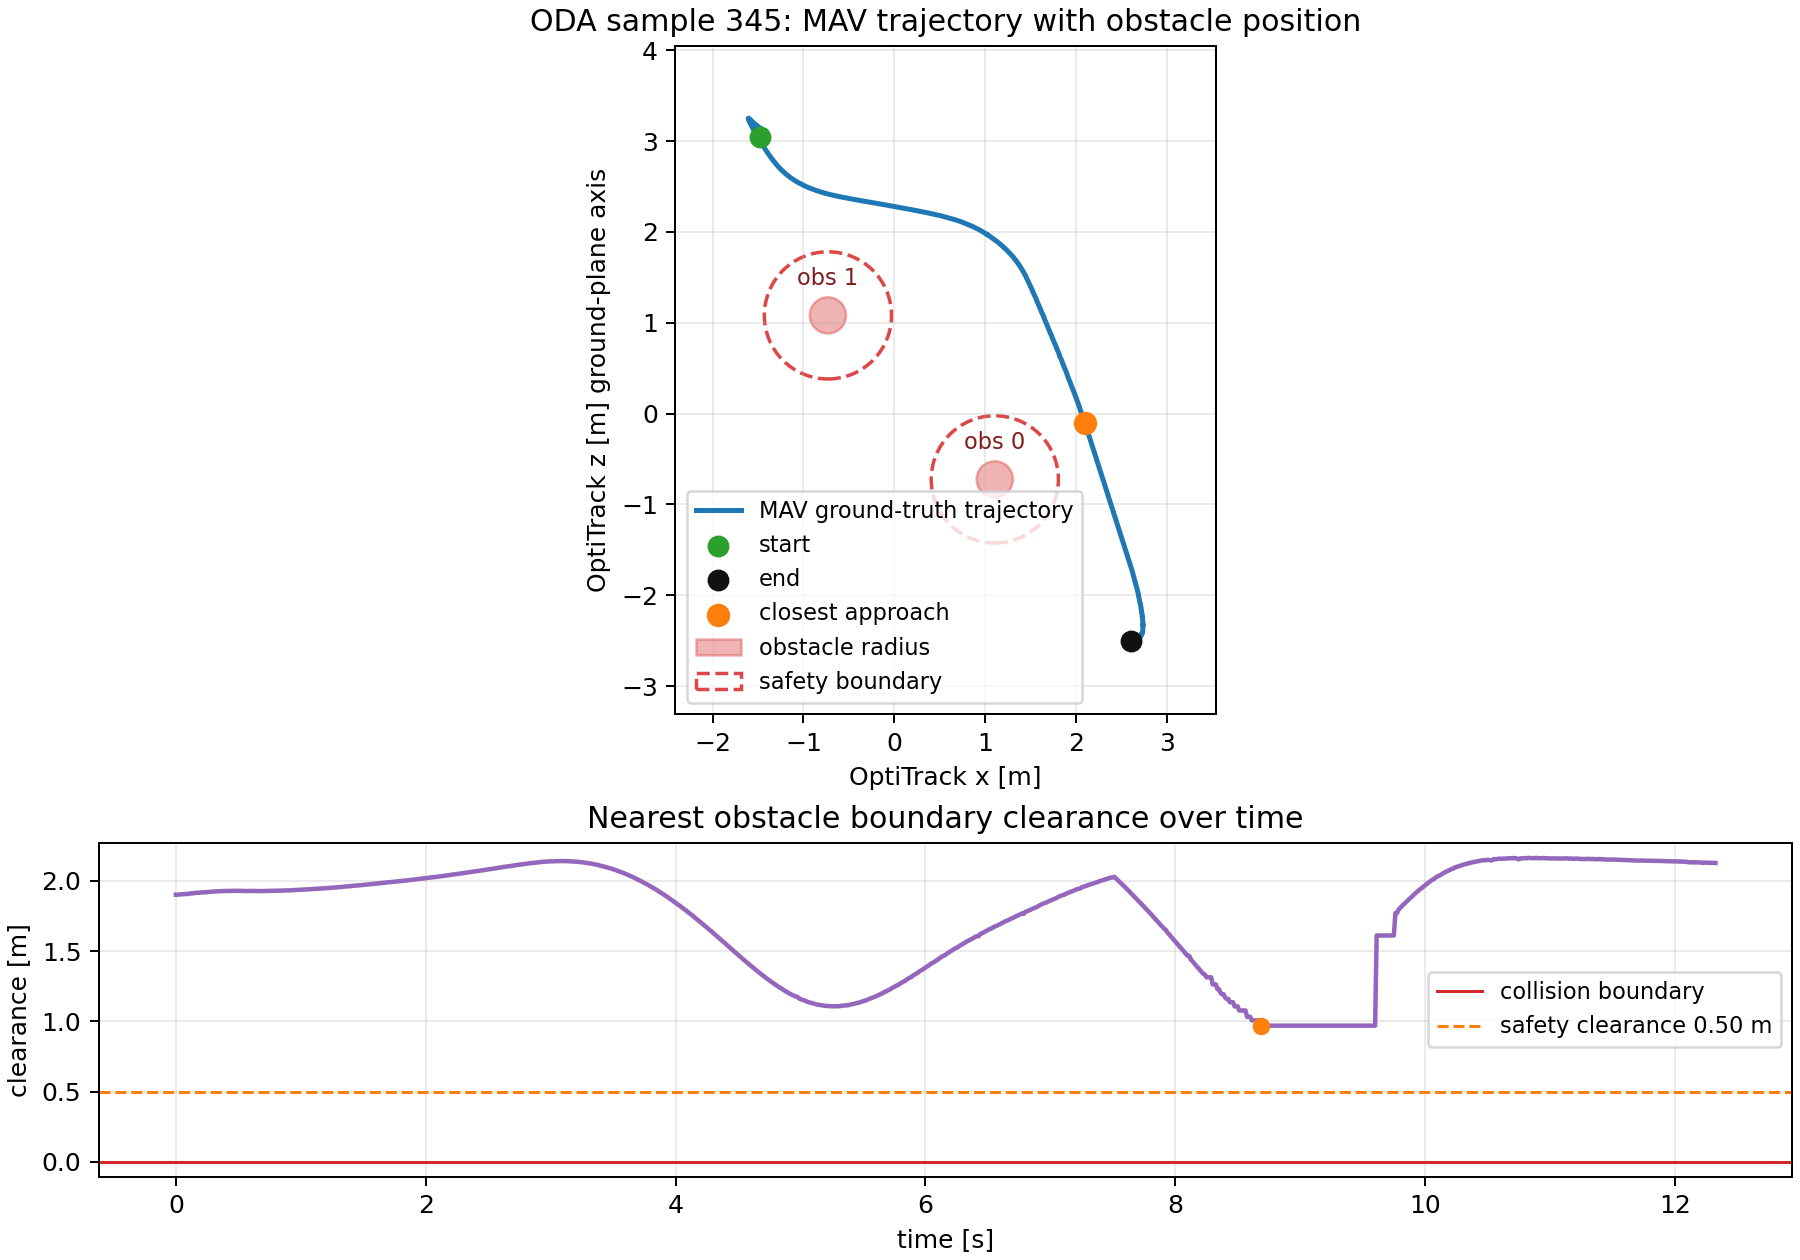
\includegraphics[width=0.49\linewidth]{trajectory_sample_345.png}
\caption{Minh họa quỹ đạo MAV, vị trí vật cản, safety boundary và clearance theo thời gian cho sample 3 và 345.}
\end{figure}

\subsection{So sánh planner baseline}
Trên ba trial local đã đủ OptiTrack/RGB/radar/IMU, pipeline đã so sánh quỹ đạo người lái với sáu baseline: đường thẳng từ start tới goal, geometric bypass bằng waypoint tránh biên an toàn, A* trên occupancy grid 2D, RRT, RRT* và MPPI Python nhẹ. Bảng dưới đây là kết quả batch benchmark mới nhất.

\begin{table}[H]
\centering
\small
\caption{So sánh quỹ đạo người lái và planner baseline trên các sample 3, 10 và 345.}
\begin{tabular}{l r r r r r}
\toprule
Phương pháp & Trial & Collision rate & Violation rate & Mean clearance (m) & Mean compute (ms) \\
\midrule
Human trajectory & 3 & 0.0000 & 0.3333 & 0.7446 & 0.0000 \\
Straight-line & 3 & 0.3333 & 0.6667 & 0.4055 & 1.6204 \\
Geometric bypass & 3 & 0.0000 & 0.0000 & 0.7386 & 2.7720 \\
A* grid planner & 3 & 0.0000 & 0.0000 & 0.6092 & 5.6578 \\
RRT & 3 & 0.0000 & 0.0000 & 0.6343 & 8.6344 \\
RRT* & 3 & 0.0000 & 0.0000 & 0.6360 & 75.5094 \\
MPPI & 3 & 0.0000 & 0.0000 & 0.7386 & 4.4417 \\
\bottomrule
\end{tabular}
\end{table}

Kết quả cho thấy baseline đường thẳng có quãng đường ngắn hơn nhưng không an toàn: collision rate đạt \(0.3333\) và safety-violation rate đạt \(0.6667\). Geometric bypass, A*, RRT, RRT* và MPPI loại bỏ collision/safety violation trên cả ba trial local. RRT* hiện chậm hơn do là prototype Python chưa tối ưu, còn MPPI được warm-start từ geometric bypass để tạo baseline tối ưu hóa nhẹ. Điều này tạo cơ sở định lượng để mở rộng so sánh planner sau khi có thêm trial từ full dataset.

\begin{figure}[H]
\centering
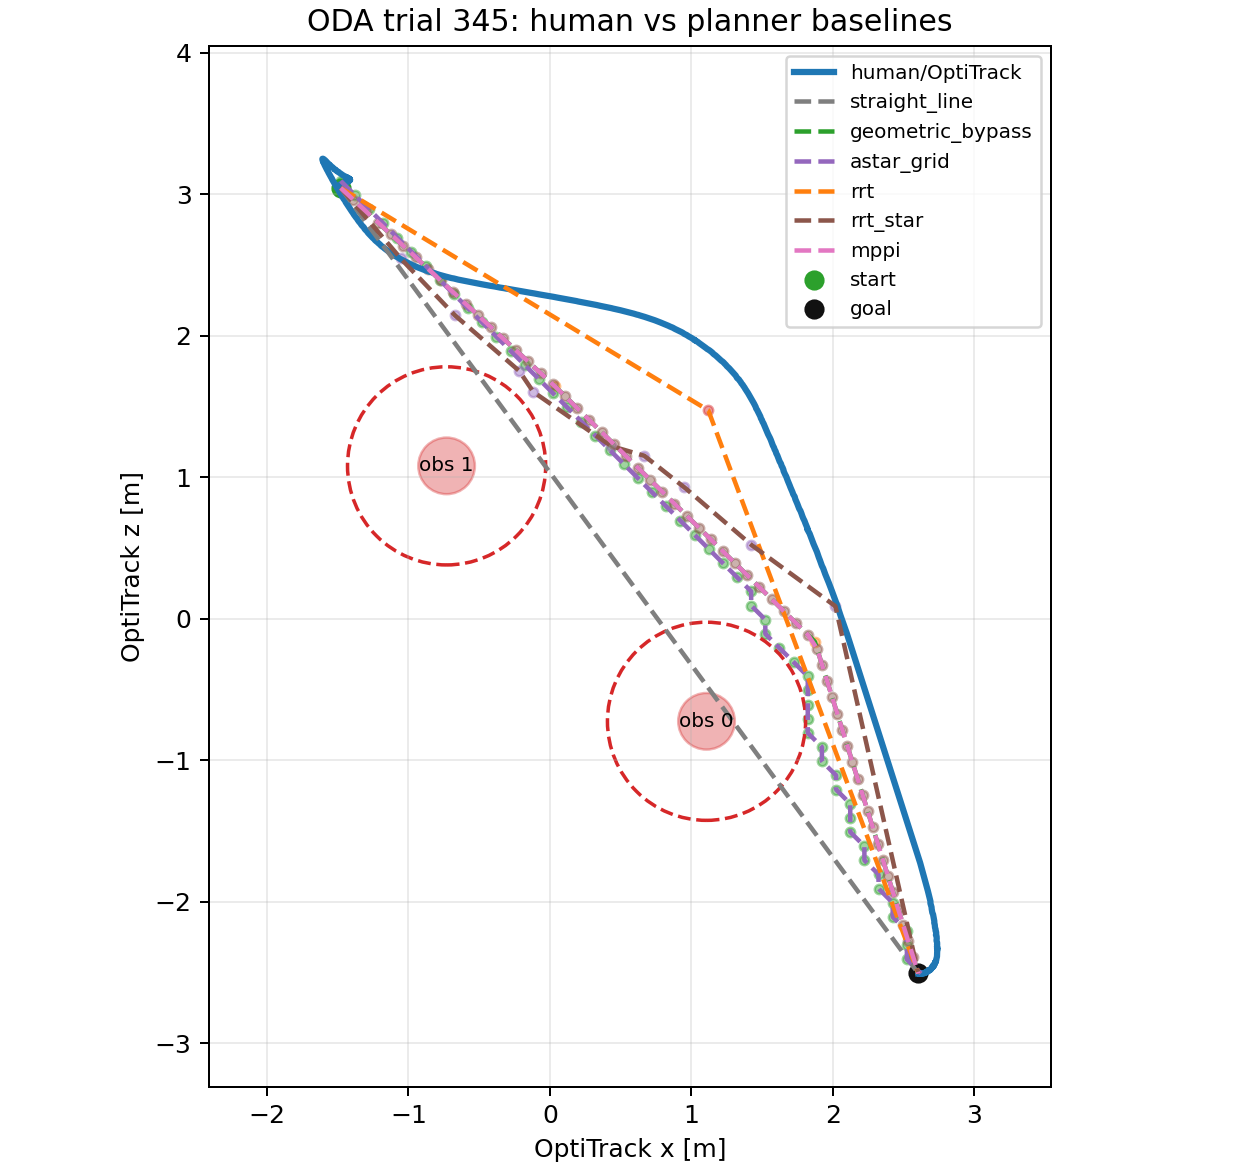
\includegraphics[width=0.82\linewidth]{planner_comparison_sample_345.png}
\caption{So sánh human trajectory, straight-line, geometric bypass, A*, RRT, RRT* và MPPI trên sample 345 có hai vật cản.}
\end{figure}

\subsection{Kết quả định tính}
Các video MP4 đã được xuất tại \texttt{outputs/videos/}. Hai video hoàn chỉnh nhất là:
\begin{itemize}
  \item \texttt{qualitative\_depth\_sensor\_sample\_3.mp4}: RGB + predicted depth + radar FFT + IMU + safety map + trajectory; thể hiện case vi phạm khoảng cách an toàn.
  \item \texttt{qualitative\_depth\_sensor\_sample\_345.mp4}: cùng cấu trúc 6 panel cho case hai vật cản.
\end{itemize}

\begin{figure}[H]
\centering
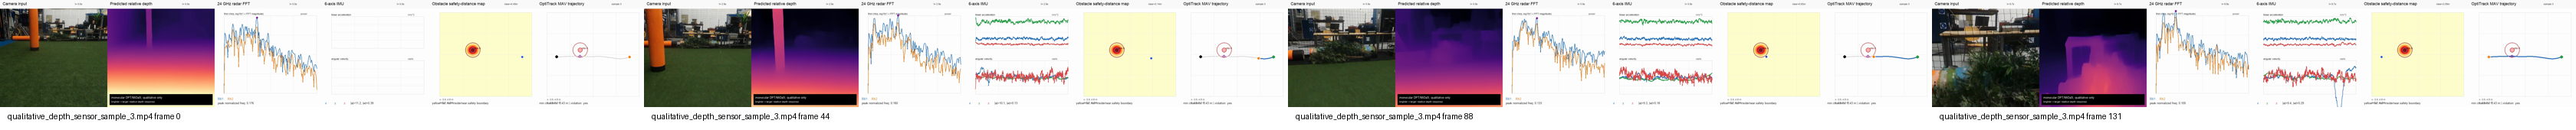
\includegraphics[width=\linewidth]{qualitative_depth_sensor_sample_3_contact_sheet.png}
\caption{Contact sheet của video 6 panel cho sample 3: RGB, relative depth, radar FFT, IMU, safety map và trajectory.}
\end{figure}

\subsection{Đính kèm mã nguồn và bộ cài}
Mã nguồn và script tái lập kết quả nằm trong cùng thư mục dự án. Các lệnh chính:
\begin{lstlisting}[basicstyle=\ttfamily\small,breaklines=true,frame=single]
scripts/fetch_oda_minimal.sh
scripts/fetch_oda_video_sample.sh data/raw/ODA_Dataset 3
scripts/fetch_oda_sensor_sample.sh data/raw/ODA_Dataset 3
scripts/cache_oda_depth_sample.sh 3
python3 experiments/benchmark_oda.py
python3 experiments/make_qualitative_video.py --trial-id 3 --include-depth --include-sensors --output outputs/videos/qualitative_depth_sensor_sample_3.mp4
\end{lstlisting}

\section{Đánh giá hiệu quả}
\begin{table}[H]
\centering
\small
\caption{Đánh giá theo các tiêu chí phù hợp với yêu cầu chấm điểm.}
\begin{tabularx}{0.96\linewidth}{>{\bfseries}p{3.0cm} X}
\toprule
Tiêu chí & Đánh giá \\
\midrule
Độ khó và phức tạp & Bài toán kết hợp UAV indoor, dữ liệu đa cảm biến, motion-capture ground truth, metric an toàn và trực quan hóa theo thời gian. \\
Quy mô công việc & Đã triển khai pipeline đọc dữ liệu, benchmark metric, hình tĩnh, video 3/5/6 panel, depth cache và script tái lập. \\
Tính sáng tạo & Không chỉ chạy visualization gốc mà tái cấu trúc thành framework benchmark: risk label, safety map, planner baseline, radar FFT, IMU rolling plot, predicted depth và trajectory trong cùng video. \\
Mức độ hoàn thiện & Có output cụ thể: bảng CSV, hình PNG, video MP4, mã nguồn module hóa, batch benchmark human-vs-planner và lệnh reproduce. Full benchmark 20 trial đang phụ thuộc vào việc tải/extract full archive 4TU. \\
Hiệu quả tính toán & Metric trajectory chạy dưới \(1\,ms\)/trial; depth được cache ở 5 fps để render lại video nhanh, tránh inference lại nhiều lần. \\
\bottomrule
\end{tabularx}
\end{table}

So với cách tiếp cận khảo sát lý thuyết đơn thuần, pipeline hiện tại tạo được kết quả chạy được và có số liệu kiểm chứng. So với việc bắt đầu bằng ROS/Gazebo hoặc mô hình học sâu nặng, cách làm này giảm rủi ro triển khai, phù hợp để trình bày kết quả sớm và làm nền cho so sánh planner.

\section{Kết luận}
Đề tài đã đạt được mục tiêu giai đoạn đầu: xây dựng pipeline nhẹ trên ODA Dataset, tái dựng quỹ đạo MAV với vật cản, tính metric an toàn, tạo nhãn rủi ro, xuất video định tính đa cảm biến và so sánh quỹ đạo thật với các planner baseline. Tính mới của sản phẩm nằm ở việc biến các sample rời rạc của dataset thành một quy trình benchmark có thể mở rộng: từ metadata/ground truth tới risk label, radar, IMU, relative monocular depth và planner comparison. Tính hiệu quả thể hiện ở việc có kết quả số, hình và video minh chứng cụ thể chỉ với pipeline Python nhẹ.

Hướng phát triển tiếp theo gồm: tải hoặc extract thêm các trial mục tiêu từ full archive 4TU để chạy đủ benchmark 20 trial, sau đó chạy RRT*/MPPI với cấu hình server đầy đủ và mở rộng perception-risk bằng depth/radar/IMU. Riêng depth panel cần được đánh giá độ ổn định theo thời gian và hiệu chuẩn với ground truth/radar trước khi dùng như metric depth; ROS/Gazebo và các controller nặng nên để sau khi benchmark ODA ổn định.

\renewcommand{\refname}{Tài liệu tham khảo}
\begin{thebibliography}{9}
\bibitem{odaGithub}
J. Dupeyroux, R. Dinaux, N. Wessendorp, and G. de Croon, ``ODA Dataset GitHub Repository,'' \url{https://github.com/JuSquare/ODA_Dataset}.

\bibitem{oda4tu}
J. Dupeyroux, R. Dinaux, N. Wessendorp, and G. de Croon, ``The Obstacle Detection and Avoidance Dataset for Drones,'' 4TU.ResearchData, DOI: \url{https://doi.org/10.4121/14214236.v1}.

\bibitem{odaPaper}
J. Dupeyroux, R. Dinaux, N. Wessendorp, and G. C. H. E. de Croon, ``A Novel Obstacle Detection and Avoidance Dataset for Drones,'' 2022. \url{https://research.tudelft.nl/en/publications/a-novel-obstacle-detection-and-avoidance-dataset-for-drones/}.

\bibitem{dptPaper}
R. Ranftl, A. Bochkovskiy, and V. Koltun, ``Vision Transformers for Dense Prediction,'' ICCV, 2021. \url{https://arxiv.org/abs/2103.13413}.

\bibitem{dptModel}
Intel, ``DPT-Hybrid MiDaS model card,'' Hugging Face. \url{https://huggingface.co/Intel/dpt-hybrid-midas}.

\bibitem{mppi}
Rapyuta Robotics, ``MPPI Controller,'' GitHub. \url{https://github.com/rapyuta-robotics/mppi_controller}.

\bibitem{fastlivo2}
HKU-MARS, ``FAST-LIVO2,'' GitHub. \url{https://github.com/hku-mars/FAST-LIVO2}.
\end{thebibliography}

\end{document}
